\documentclass[border=5mm, convert, usenames, dvipsnames,beamer]{standalone}
\usetheme{Madrid}
\usecolortheme{default}
%Information to be included in the title page:
\title{Sample title}
\author{Anonymous}
\institute{Overleaf}
\date{2021}

\usepackage[absolute,overlay]{textpos}

\defbeamertemplate*{frametitle}{}[1][]
{
    \begin{textblock*}{8cm}(1cm,0.55cm)
    {\color{purple} \fontsize{16}{24} \selectfont \insertframetitle}
    \end{textblock*}
    \begin{textblock*}{12cm}(1cm,2.5cm)
    {\color{purple} \fontsize{20}{24} \selectfont \insertframesubtitle}
    \end{textblock*}
}


\usepackage{ragged2e}

\justifying
\usepackage{lmodern}
\usepackage{ImageMagick}
\usepackage[utf8] {inputenc}
\usefonttheme[onlymath]{serif}
\usepackage[english] {label}
\usepackage{amssymb}
\usepackage{amsmath}
\usepackage{bm}
\usepackage{bbm}
\usepackage[round] {natbib}
\usepackage{color}     
\usepackage{changepage}
\usepackage[export]{adjustbox}
\usepackage{graphicx}
\usepackage{minted}
\usepackage{listings}
\usepackage[svgnames]{xcolor}
\makeatletter
\newcommand\listofframes{\@starttoc{lbf}}
\makeatother

\setbeamertemplate{footline}[frame number]

\lstdefinestyle{R} {language=R,
    stringstyle=\color{DarkGreen},
    morekeywords={TRUE,FALSE},
    deletekeywords={data,frame,length,as,character},
    keywordstyle=\color{blue},
    commentstyle=\color{teal},    
    basicstyle=\ttfamily\tiny,
    breakatwhitespace=false,         
    breaklines=true,                 
    captionpos=b,                    
    keepspaces=true,                 
    numbers=left,                    
    numbersep=3pt,                  
    showspaces=false,                
    showstringspaces=false,
    showtabs=false,                  
    tabsize=1
}

\definecolor{codegreen}{rgb}{0,0.6,0}
\definecolor{codegray}{rgb}{0.5,0.5,0.5}
\definecolor{codepurple}{rgb}{0.58,0,0.82}

\lstdefinestyle{Python} {language=Python,
    commentstyle=\color{codegreen},
    keywordstyle=\color{magenta},
    numberstyle=\tiny\color{codegray},
    stringstyle=\color{codepurple},
    basicstyle=\ttfamily\tiny,
    breakatwhitespace=false,         
    breaklines=true,                 
    captionpos=b,                    
    keepspaces=true,                 
    numbers=left,                    
    numbersep=3pt,                  
    showspaces=false,                
    showstringspaces=false,
    showtabs=false,                  
    tabsize=1}




\def\one{\mbox{1\hspace{-4.25pt}\fontsize{12}{14.4}\selectfont\textrm{1}}} % 11pt 

\makeatletter
\setbeamertemplate{frametitle}[default]{}
\makeatother
\usepackage{booktabs}
\newcommand{\ra}[1]{\renewcommand{\arraystretch}{#1}}


\begin{document}




\end{frame}

\begin{frame}
\frametitle{Poisson Likelihood}
\listofframes

\vspace{40}
\noindent
Suppose that a r.v. $X$ obeys a Poisson distribution $\mathcal{P}(\lambda)$, characterized by the following Probability Mass Function (PMF)

$$
f_{\lambda}(x) = \frac{\lambda^{x}e^{- \lambda}}{x!}
$$

\vspace{5}
\noindent
If we observe a sample $x_{1},...,x_{n}$, then the likelihood is just the product of the individual PMF

$$
\begin{align*}
\pi( x_{1},...,x_{n}  \mid \lambda ) & =\frac{\lambda^{\sum_{i=1}^{n} x_{i}}e^{- n \lambda}}{\prod_{i=1}^{n} ( x_{i}!)} \\
& =\frac{\lambda^{n \bar{x}}e^{- n \lambda}}{\prod_{i=1}^{n} ( x_{i}!)} \\
\end{align*}
$$

\vspace{5}
\noindent
where the model parameter $\lambda$ is the count of some event of interest and $\bar{x} = \frac{1}{n} \sum_{i=1}^{n} x_{i}$.


\par
\end{frame}




\begin{frame}[ fragile]{}
\frametitle{Some examples of Poisson samples}
\vspace{50}
\noindent

 \includegraphics[scale=0.54,center]{plotR0}


\end{frame}








\begin{frame}[ fragile]{}

\frametitle{Gamma prior}

\vspace{30}
\noindent
 A convenient choice to model the uncertainty about $\lambda$ is a Gamma distribution as prior, since the support of such a distribution is the interval $[0, \infty[$. A Gamma prior with shape parameter $\alpha$ and scale parameter $\beta$ has the following form

$$
\pi( \lambda) =  \frac{  \beta^{\alpha}   }{ \Gamma(\alpha)  } \lambda^{\alpha - 1}   e^{- \lambda \beta }
$$

\vspace{5}
\noindent
where $\Gamma(\alpha)$ is the Gamma function, defined as $\int_{0}^{\infty}x^{\alpha - 1}  e^{-x}  dx = (\alpha - 1) !$. 

\vspace{5}
\noindent
Let $X \sim Gamma(\alpha, \beta)$. Then $E[X]= \alpha/ \beta$ and $var(X)=\alpha /\beta^2$.

\vspace{5}
\noindent
It is a convenient and flexible choice since the Gamma distribution can take a wide variety of shapes.





\end{frame}






\begin{frame}[ fragile]{}
\frametitle{Some examples of the Gamma family}

\vspace{50}
\noindent

 \includegraphics[scale=0.54,center]{plot1R}


\end{frame}




\begin{frame}
\frametitle{Gamma posterior (1/2)}

\vspace{40}
\noindent
The posterior distribution for $\lambda$ if our data $x_{1},...,x_{n}$ is modeled with a Poisson likelihood and a Gamma prior is chosen for $\lambda$ will also have the functional form of a Gamma r.v. Using the Bayes theorem, we have that

$$
\begin{align*} 
 \pi(\lambda \mid x_{1},...,x_{n}) & =  \frac{\pi( x_{1},...,x_{n} \mid \lambda) \pi( \lambda) }{\pi(x_{1},...,x_{n})} \\
&  =\frac{\lambda^{n \bar{x}}e^{- n \lambda}}{\prod_{i=1}^{n} ( x_{i}!)} \frac{  \beta^{\alpha}   }{ \Gamma(\alpha)  } \lambda^{\alpha - 1}   e^{- \lambda \beta } \\
 & = \underbrace{\frac{1}{\prod_{i=1}^{n} ( x_{i}!)}   \frac{  \beta^{\alpha}   }{ \Gamma(\alpha)  }}_{\text{do NOT depend on $\lambda$}} \  \lambda^{n \bar{x}} e^{-n \lambda} \lambda^{\alpha - 1} e^{-\lambda \beta }     \\
&  \propto   \lambda^{\alpha +n \bar{x} - 1} e^{-(n+\beta) \lambda} \\
\end{align*}
$$



\par
\end{frame}




\begin{frame}
\frametitle{Gamma posterior (2/2)}

\vspace{30}
\noindent
So we find that $\pi(\lambda \mid x_{1},...,x_{n})$ \propto Gamma(\alpha + n \bar{x}, n + \beta)$. The posterior mean and variance are given by

$$
E[\lambda] = \frac{\alpha + n \bar{x}}{n + \beta} \ \ \ \ \ \ \  var(\lambda) = \frac{\alpha + n \bar{x}}{(n + \beta)^{2}}
$$

\vspace{5mm}
\noindent
where $n \bar{x} =  \sum_{i=1}^{n} x_{i}$ is the sum of the counts and $n$ is the sample size. Let's take a few examples and plot the likelihood, a possible prior and the posterior, all at once in R.


\par
\end{frame}



\begin{frame}
\frametitle{General remark on Bayesian inference}

\vspace{40}
\noindent
Unlike in the traditional Frequentist framework, the Bayesian approach views parameters as random variables rather than fixed, unknown quantities. Given a Poisson sample 
$x_{1},...,x_{n}$ and a Poisson parameter $\lambda$, from the Bayes theorem, we can write 

$$
\pi(\lambda \mid x_{1},...,x_{n}) = \frac{\pi( x_{1},...,x_{n}  \mid \lambda ) \  \pi( \lambda)}{ \pi(x_{1},...,x_{n})  }  
$$

\noindent
Adopting the 'proportional' notation, the constant term in the denominator is dropped so that the above expression is rewritten as $\pi(\lambda \mid x_{1},...,x_{n}) \propto  \pi( x_{1},...,x_{n}  \mid \lambda ) \  \pi( \lambda)$

\vspace{5}
\noindent
When conjugate models are used (as in the case of a Poisson-Gamma model), the posterior distribution can be identified and closed-form quantities of interest like a mean, a variance or quantiles can be computed. Most of the time in practice, the posterior distribution is intractable so that it is necessary to resort to MCMC techniques.


\par
\end{frame}




\begin{frame}
\frametitle{Working example}

\vspace{30}
\noindent
Suppose that we record the number of a specific bacteria present in 20 water samples taken in the Mekong Delta (Vietnam) so that we have the following data at hand:

$$
x_{i} = 1, 0, 0, 1, 0, 0, 1, 1, 0, 1, 2, 0, 0, 5, 2, 0, 0, 2, 0, 1
$$

\vspace{10}
\noindent
So assuming a Poisson likelihood with parameter $\lambda =1$, namely a $\mathcal{P}(1)$ likelihood for the data and using a $Gamma(2,2)$ prior, with mean $2/2=1$ and variance $2/2^2 = 0.5$, what is the posterior mean and the $95 \%$ credible intreval for the model parameter?



\par
\end{frame}





\begin{frame}[ fragile]{}
\frametitle{Working example: posterior}

\vspace{50}
\noindent

 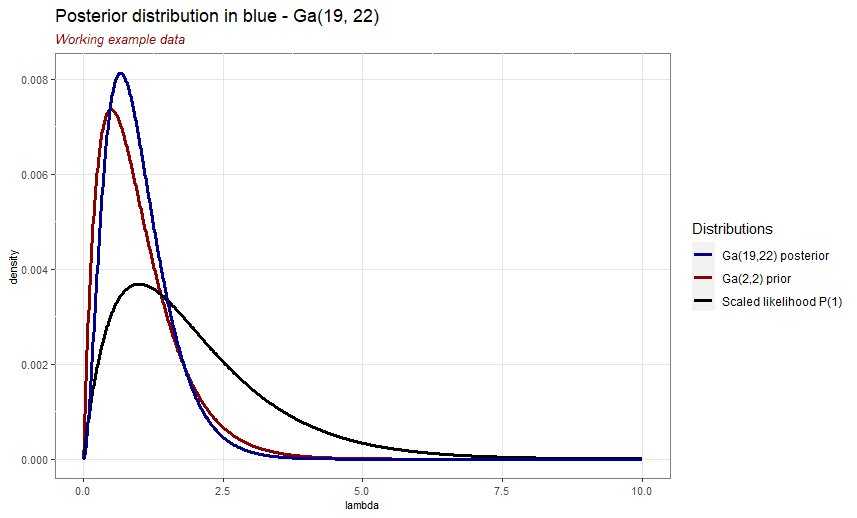
\includegraphics[scale=0.50,center]{posterior}


\end{frame}





\begin{frame}[ fragile]{}

\frametitle{Posterior quantities obtained from direct sampling}

\vspace{50}
\noindent

\tiny
\par

\begin{lstlisting}[style=
R]
# Posterior mean, posterior variance and 95% Credible Interval including the sample median
set.seed(2023)
data1 = rpois(n = n, lambda = lambda1)
alpha_posterior = round(alpha1 + n*mean(data1), 2) # 19
beta_posterior = n + beta1 # 22

pmean = alpha_posterior / beta_posterior
pmean
# [1] 0.8636364

pvariance = alpha_posterior / beta_posterior^2
pvariance
# [1] 0.0392562

# 95% Credible Interval obtained by direct sampling (simulation)
set.seed(2023)
round(quantile(rgamma(n = 10^8, alpha_posterior, beta_posterior), probs = c(0.025, 0.5, 0.975)),4)
#   2.5%    50%  97.5% 
# 0.5200 0.8486 1.2931 

# Posterior mean obtained from direct sampling
set.seed(2023)
mean(rgamma(n = 10^8, alpha_posterior, beta_posterior))
# [1] 0.8928863
\end{lstlisting}




\par
\end{frame}



\begin{frame}
\frametitle{Jeffreys' prior: definition}

\vspace{35
}
\noindent
Let us first give the general deffinition of the Jeffreys' prior $p_{J}(\theta)$:

$$
p_{J}(\theta) = \sqrt{\mathcal{I}_{n}(\theta)}
$$

\noindent
where $\mathcal{I}_{n}(\theta)$ is the Fisher information of the sample. The Fisher information is defined as follows:

$$
 \mathcal{I}_{n}(\theta) = -E_{\theta} \left[ \frac{ \partial^{2} ln \mathcal{L}(\theta \mid \textbf{x} )} {\partial \theta^{2}}  \right]
$$

\noindent
or equivalently

$$
 \mathcal{I}_{n}(\theta) = var_{\theta} \bigg( \frac{ \partial ln\mathcal{L}(\theta \mid \textbf{x})} {\partial \theta}  \bigg) = E _{\theta}\left[ \bigg(\frac{ \partial ln\mathcal{L}(\theta \mid \textbf{x})} {\partial \theta}\bigg)^{2} \right]
$$

\noindent
The first derivative of the log-likelihood function with respect to the model parameter $\frac{ \partial ln\mathcal{L}(\theta \mid \textbf{x})} {\partial \theta}$ is sometimes referred to as the score function.

\par
\end{frame}





\begin{frame}[ fragile]{}

\frametitle{Likelihood and derived functions for \\ a Poisson model}


\vspace{20mm}
\noindent
Likelihood and log-likelihood, score function and second derivative of the log-likelihood function for a Poisson model:


\begin{align*} 
& \mathcal{L}(\lambda \mid \textbf{x} ) =  \prod_{i=1}^{n} f_{\lambda}(x_{i}) = \prod_{i=1}^{n}  \frac{\lambda^{x_{i}} e^{- \lambda}}{x_{i} !}  =  
  \frac{\lambda^{ \sum_{i=1}^{n} x_{i}} e^{- n \lambda}}{ \prod_{i=1}^{n} x_{i} !}                            \\
& l(p \mid \textbf{x} ) = ln \big( \mathcal{L}(\lambda \mid \textbf{x} ) \big) =    \sum_{i=1}^{n} x_{i} \  ln(\lambda) + - n \lambda -  \sum_{i=1}^{n} log(x_{i}!)
    \\
& \frac{ \partial ln\mathcal{L}(\lambda \mid \textbf{x})} {\partial \lambda} =  \frac{ \sum_{i=1}^{n} x_{i}}{\lambda} - n  \\
&  \frac{ \partial^{2} ln \mathcal{L}(\lambda \mid \textbf{x} )} {\partial \lambda^{2}}=    - \frac{\sum_{i=1}^{n} x_{i}}{ \lambda^{2}}    \\
\end{align*}
$$

\par
\end{frame}




\begin{frame}[ fragile]{}

\frametitle{Fisher information and Jeffrey's prior \\ for a Poisson model (1/2)}

\vspace{10mm}
\noindent
So we want

$$
 \mathcal{I}_{n}(\lambda) = -E\left[ \frac{ \partial^{2} ln \mathcal{L}(\theta \mid \textbf{x} )} {\partial \lambda^{2}}  \right]
$$

\noindent
and we note that
$$  E \bigg[   \sum_{i=1}^{n}x_{i} \bigg] = E[n  \overline{x}]     = n  E [\overline{x}] = n \lambda $$  



\par
\end{frame}



\begin{frame}[ fragile]{}
\frametitle{Fisher information and Jeffrey's prior \\ for a Poisson model (2/2)}

\vspace{55}
\noindent
Thus we have that

$$
\begin{align*} 
& \mathcal{I}_{n}(\lambda) = \frac{E \bigg[   \sum_{i=1}^{n}x_{i} \bigg] }{ \lambda^{2}}  \\
& \ \ \ \ \ \   = \frac{n \lambda}{ \lambda^{2}}   \\
& \ \ \ \ \ \   = \frac{n  }{\lambda }     \\
& \ \ \ \ \ \   \propto \lambda^{-1} \\
\end{align*}
$$

\noindent
And we conclude that

$$
p_{J}(\lambda) = \sqrt{\mathcal{I}(\lambda
)}  \propto  \lambda^{-1/2}
$$

\noindent
which is the Gamma distribution $Gamma(1/2, 0)$ (improper prior)

\par
\end{frame}



\begin{frame}[ fragile]{}

\frametitle{Gamma Jeffreys prior}

\vspace{30}
\noindent


 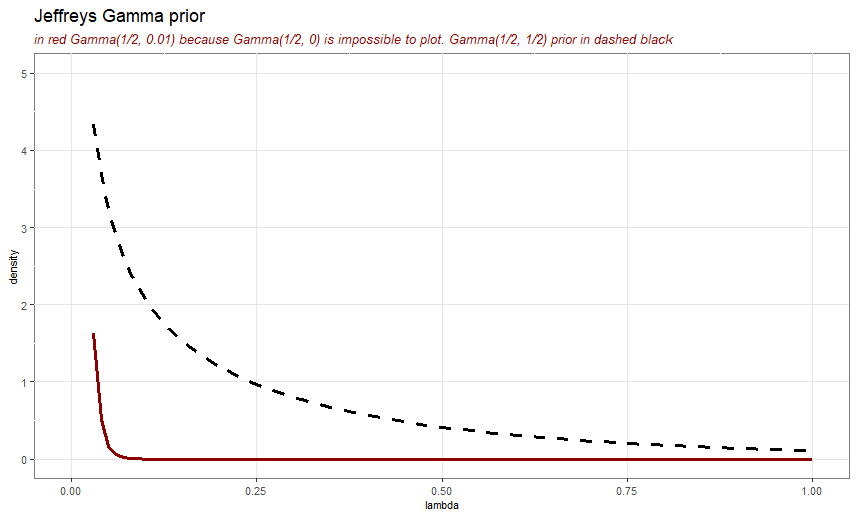
\includegraphics[scale=0.50,center]{jeffreys}



\end{frame}










\begin{frame}[ fragile]{}
\frametitle{Back to the working example (1/2
)}

\vspace{30}
\noindent
Getting back to our water samples data

$$
x_{i} = 1, 0, 0, 1, 0, 0, 1, 1, 0, 1, 2, 0, 0, 5, 2, 0, 0, 2, 0, 1
$$

\vspace{10}
\noindent
Assuming a Poisson likelihood for the data and using weakly informative prior close to the Jeffreys  prior, namely a $Gamma(1/2, 1/2)$, what is the posterior mean and the $95 \%$ credible intreval for the model parameter ?

\par
\end{frame}







\begin{frame}[ fragile]{}
\frametitle{Back to the working example (2/2)}

\vspace{40}
\noindent
From the Bayes Theorem, we know that 

$$
p( \lambda   \mid x  ) = \frac{p(x \mid \theta) \  p(\theta)}{ p(x) }  \propto  p( x   \mid \theta) \  p(\theta) 
$$

\vspace{5}
\noindent
In our case, we have that

$$
\begin{align*}
p( \lambda   \mid x  ) & \propto  \underbrace{ \lambda^{\sum_{i=1}^{n}x_{i}} e^{-10\lambda}}_{\text{Poisson  Likelihood}} \    \underbrace{ p(\lambda)}_{\text{ Prior}} \\
& \propto   \lambda^{17} e^{-20\lambda} \  \lambda^{ -1/2 }   e^{- 1/2 \lambda  } \\
& \propto   \lambda^{-16.5} \    e^{-  19.5 \lambda  } \\
\end{align} 
$$

\vspace{5}
\noindent
and we recognize the functional form of a Gamma density, that is $Gamma(\alpha = 17.5, \beta = 19.5)$. The posterior mean is given by $\alpha / \beta = 0.8974$.


\par
\end{frame}




\begin{frame}[ fragile]{}
\frametitle{Working example: in conclusion}

\vspace{30}
\noindent
So the theoretical posterior mean is given by

$$
E[\lambda] =  \frac{\alpha + n \bar{x}}{n + \beta}  =  \frac{2 + 20 *0.85}{20 + 2} = 19/22 = 0.8636364
$$

\vspace{5}
\noindent
By direct sampling, using 108 number of simulations, the posterior sample mean is $0.8636725$. 

\vspace{5}
\noindent
By direct sampling, a $95\%$ Credible Interval is given by $$[−0.5200, 1.2931]$$

\vspace{10}
\noindent
So, combining modeling and simulations, we are now able to generalize and infer to the whole population of bacteria in the Mekong Delta those values from a sample of size 20.


\end{frame}








\begin{frame}[ fragile]{}
\frametitle{Further reading and code}


\vspace{0}
\noindent
The R Project for Statistical Computing:

\noindent
\urlf{https://www.r-project.org/}


\vspace{10}
\noindent
Accessing the R code:

\noindent
\urlf{https://github.com/JRigh/Poisson-Gamma-example-in-R/blob/main/ \\
Poisson-Gamma%20R%20code}




\par
\end{frame}










\end{document}
